% !TeX root = Bericht_main.tex
\subsection{Aufgabe 35}
Wir betrachten nochmals das Regenwasserversickerungsproblem aus den ersten Übungsblättern und wollen im Folgenden vorallem die Genauigkeit von linearen, quadratischen und DG-Ansatzelementen
vergleichen. Dazu betrachten wir das gleiche Problem auf unterschiedlichen Leveln für die unterschiedlichen Ansätze. Wir  wollen vorallem die Größen Outflow, Flux Error, Flux Loss vergleichen und zusätzlich mit den Größen Problem Size und Programmdauer auf den Faktor Effizienz eingehen.

\subsubsection{Aufgabe 35.1}
In einem ersten Schritt wollen wir den Einfluss der Wahl der Ansatzelemente beim Finiten Elemente Verfahren untersuchen.
Wir betrachten dazu die entsprechenden Lösungen für lineare Ansatzelemente (Discretization = linear) und quadratische Ansatzelemente (Discretization = serendipity) bei ähnlicher Problemgröße.
\begin{figure}[H]
	\centering
	\captionabove{Discretization = linear}
	\subfigure{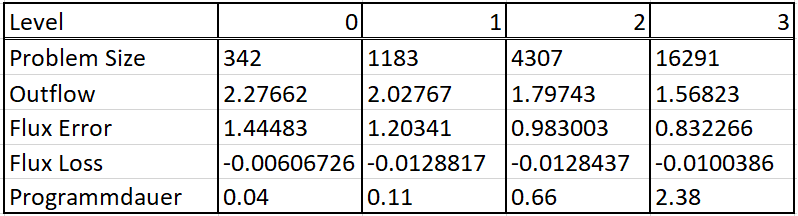
\includegraphics[width=0.99\textwidth]{../Aufgabe35/35_1_linear.png}}	 
\end{figure}

\begin{figure}[H]
	\centering
	\captionabove{Discretization = serendipity}
	\subfigure{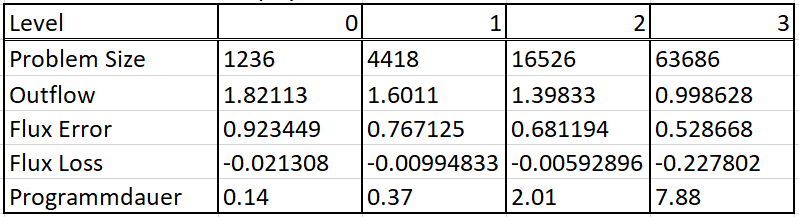
\includegraphics[width=0.99\textwidth]{../Aufgabe35/35_1_serendipity.png}}	 
\end{figure}
Man sieht sehr leicht, dass bei ähnlicher Problemgröße die quadratischen Ansatzelemente den linearen Ansatzelementen überlegen sind. Beispielsweise liefert der lineare Ansatz auf Level 1 (Problemgröße $\approx$ $1200$) einen Flux Error von $\approx 1.2$, während der quadratische Ansatz aus Level 0 (ebenfalls Problemgröße $\approx$ $1200$) mit einem Flux Error von $\approx 0.92$ genauer ausfällt. Diese Erkenntnis zieht sich auch bei anderen Wertepaaren durch die Tabelle.
Wir können dies auch von theoretischer Seite aus erklären:

Sei $V$ der Ansatzraum und $a(\cdot,\cdot)$ die zugehörige Bilinearform unseres aktuell gewählten Verfahrens (Finite Elemente bzw. Discontinuous Galerkin).
Wir erhalten dann im folgenden Lemma eine Aussage über die Güte unserer Approximationslösung:

\begin{Lemma}[Cea's Lemma]
  Sei $a(\cdot,\cdot)$ beschränkt und elliptisch, d.h.
  \begin{align*}
    |a(u,v)| \le C \|u'\| \|v'\|, \quad a(u,v) \ge c \| v'\|^2
    \quad \forall u,v \in V.
  \end{align*}
  Dann gilt für den Galerkin-Fehler $e_h = u-u_h$
  \begin{align*}
    \| e_h' \| \le \frac{C}{c} \inf\limits_{v_h \in V}
    \| u'-v_h' \|.
  \end{align*}
\end{Lemma}
Mit anderen Worten heißt das: Die berechnete Galerkin Approximation ist bezüglich einer geeigneten Norm eine Bestapproximation in unserem Ansatzraum $V$.
Die Vorraussetzungen des obigen Lemmas sind sowohl für die FEM als auch für das DGV erfüllt (vgl. Bericht 1-3 und
\textcolor{green}{ ? siehe Theorie }
Wir erhalten deshalb für quadratische Ansatzelemente auch eine etwas bessere Lösung, denn der Ansatzraum $V_h^{lin}$ der linearen Ansatzelemente ist natürlich Teilmenge des Ansatzraumes $V_h^{quad}$ der quadratischen Ansatzelemente. Da es sich bei der Finite Elemente Lösung um eine Galerkin-Approximation handelt und diese nach obigem Lemma eine Bestapproximation im zugehörigen Ansatzraum darstellt, kann die Lösung im größeren Ansatzraum $V_h^{quad}$ nur besser ausfallen.

Erstaunlich ist dabei, dass die Programmdauer bei minimal größerer Problemgröße und zudem besserer Genauigkeit bei den quadratischen Ansatzelementen für ungefähr gleiche Problemgröße dennoch meist geringer ausfällt als bei linearen Ansatzelementen. Zum Beispiel liefert Level 2 bei den lineare Ansatzelementen eine Programmdauer von 0.66 Sekunden, bei den quadratischen Ansatzelementen auf Level 1 aber nur von 0.37 Sekunden (Problemgröße $\approx 4350$ bei beiden).



\subsubsection{Aufgabe 35.2}
Als nächstes wollen wir uns dem DG-Ansatz widmen. Wir vergleich hier zunächst ???
\begin{figure}[H]
	\centering
	\captionabove{symmetric}
	\subfigure{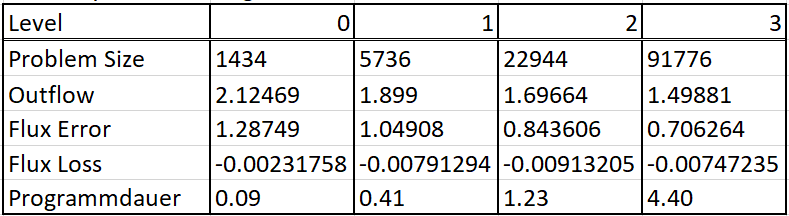
\includegraphics[width=0.99\textwidth]{../Aufgabe35/35_2_sym.png}}	 
\end{figure}

\begin{figure}[H]
	\centering
	\captionabove{non-symmetric}
	\subfigure{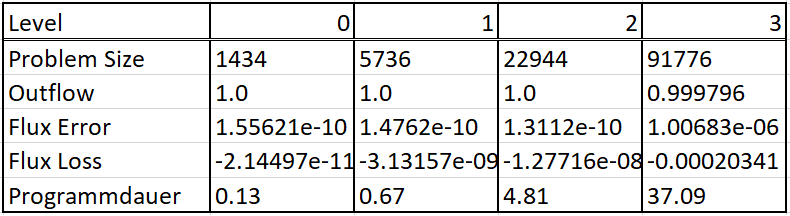
\includegraphics[width=0.99\textwidth]{../Aufgabe35/35_2_nonsym.png}}	 
\end{figure}


\subsubsection{Aufgabe 35.3}
\begin{figure}[H]
	\centering
	\captionabove{deg = 2}
	\subfigure{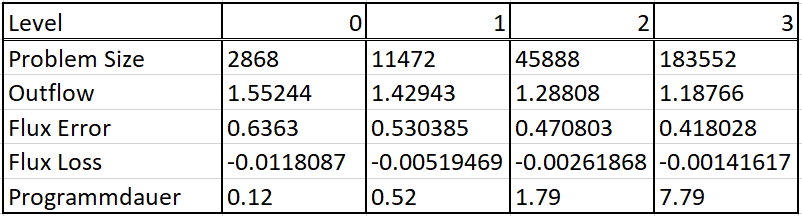
\includegraphics[width=0.99\textwidth]{../Aufgabe35/35_3_level.png}}	 
\end{figure}

\begin{figure}[H]
	\centering
	\captionabove{deg = 2, symmetrisch, level = 3}
	\subfigure{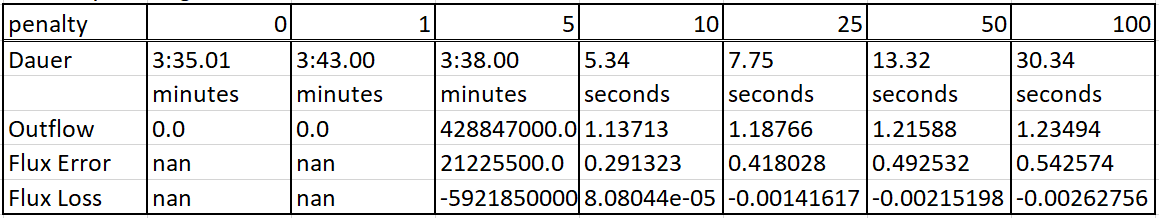
\includegraphics[width=0.99\textwidth]{../Aufgabe35/35_3_dauer.png}}	 
\end{figure}





